\documentclass[a4paper, 11pt]{article}
 



%%%%%%%%%%%%%%%%%%%%%%%%%%%%%%%%%
%	 PACKAGES	%
%%%%%%%%%%%%%%%%%%%%%%%%%%%%%%%%%
% Codierung von in und Output
\usepackage[utf8]{inputenc}
\usepackage[T1]{fontenc}

% AMS-Pakete für Mathe
\usepackage{amsthm,amssymb,amsmath}

% Sprachpaket neue rechtschreibung
\usepackage[ngerman]{babel} 


\usepackage[many]{tcolorbox}

%Header und Seitengrösse
\usepackage{fancyhdr}
\usepackage{geometry}

% Paket für Links im PDF (glaubs)!
\usepackage[hidelinks]{hyperref}

%Paket um ganze pdf-File zu importieren (Arbeitsblätter aus Analysis DMK)
\usepackage{pdfpages}

%TColorbox nutzt Theoreme und bessere Verweise
\tcbuselibrary{theorems}
\usepackage{cleveref}

%Package, um Aufgaben auf mehrere Spalten zu verteilen.
\usepackage{tasks}

% kein Plan, was das folgende macht... :(
\usepackage{listings}
\lstset{basicstyle=\ttfamily}
\makeatletter
\def\BState{\State\hskip-\ALG@thistlm}
\makeatother

\usepackage{graphicx}
\usepackage{hyperref}
\usepackage{array}
\hypersetup{colorlinks=true}

% damit kann man nummerierte Liste unterbrechen und wieder aufnehmen
\usepackage{enumitem} 

% SI einheiten
\usepackage{siunitx}

%%%CHANGE LABEL FIGURE
\usepackage[figurename=Abbildung.]{caption}
\usepackage{subcaption}

%%%%%%%%%%%%%%%%%%%%%%%%%%%%%%%%
%%%%%%%%%%%	LAYOUT	%%%%%%%%%%%%
%%%%%%%%%%%%%%%%%%%%%%%%%%%%%%%%

\geometry{
	a4paper,
	total={165mm,225mm},
	left=25mm,
	top=35mm,
}

%keine Einrückung bei Absatz dafür Abstand
\setlength\parindent{0pt}
\setlength{\parskip}{1em}

%Header
\pagestyle{fancy}
\setlength{\headheight}{13.6pt}
\renewcommand{\sectionmark}[1]{ \markright{#1}{} }
\lhead[L]{M. Anderegg}
\chead{}
\rhead{\rightmark}
\lfoot{}
\cfoot{\thepage}
\rfoot{}





%%%%%%%%%%%%%%%%%%%%%%%%%%%%%%%%
%%%%%%%%% TCB-Commands %%%%%%%%%
%%%%%%%%%%%%%%%%%%%%%%%%%%%%%%%%

\newtcbtheorem
[auto counter, number within=section, crefname={beispiel}{beispiele}, Crefname={Beispiel}{Beispiele}] % Nummerierung und Name bei Verweis
{bsp} % Name der Umgebung \begin{bsp}
{Beispiel} %Name der im Titel angezeigt wird
{breakable, enhanced, fonttitle=\bfseries, coltitle = black, colbacktitle = orange!15, righthand width=3cm,
	sharp corners,boxrule=.4pt,colback=orange!5} %%Optionen für die Box. 
	%Breakable und Enhanced lassen zu, dass sich die Box auf zwei Seiten verteilt.
{bsp} %So wird intern auf die Referenz verwiesen.

\newtcbtheorem[auto counter,  crefname={lernaufgabe}{lernaufgaben},
Crefname={Lernaufgabe}{Lernaufgaben}]{LA}{Lernaufgabe}{
	breakable, enhanced, fonttitle=\bfseries, coltitle = black, colbacktitle = cyan!15, righthand width=3cm,
	sharp corners,boxrule=.4pt,colback=white}{LA}

\newtcbtheorem[auto counter, number within=section]{ueb}{Übung}{
	breakable, fonttitle=\bfseries, coltitle = black, colbacktitle = blue!15, righthand width=3cm,
	sharp corners,boxrule=.4pt,colback=blue!5}{uebng}


\newtcbtheorem[auto counter, number within=section, crefname={definition}{definitionen},
Crefname={Definition}{Definitionen}]{definition}{Definition}{
	breakable, colframe=green!70!black, fonttitle=\bfseries, coltitle = white, colbacktitle = green!70!black, enhanced, attach boxed title to top left={yshift=-0.1in, xshift=0.15in},}{def}

\newtcbtheorem[auto counter, number within=section, crefname={Satz}{Sätze},
Crefname={Satz}{Sätze}]{satz}{Satz}{%
	breakable, lower separated=false,
	colframe=red!70!white, fonttitle=\bfseries, coltitle = white, colbacktitle = red!70!white, enhanced, attach boxed title to top left={yshift=-0.1in,xshift=0.15in},
}{satz}




%%%%%%%%%%%%%%%%%%%%%%
%%%% Mathe-Befehle %%%
%%%%%%%%%%%%%%%%%%%%%%


\newcommand{\N}{\mathbb{N}}
\newcommand{\Z}{\mathbb{Z}}
\newcommand{\Q}{\mathbb{Q}}
\newcommand{\R}{\mathbb{R}}
\newcommand{\C}{\mathbb{C}}
\newcommand{\LL}{\mathbb{L}}
\newcommand{\DD}{\mathbb{D}}
\newcommand{\Ra}{\Rightarrow}

% TikZ
\usepackage{pgfplots}	
\pgfplotsset{compat=1.8}
\usepackage{pgf,tikz}
\usepackage{mathrsfs}
\usetikzlibrary{arrows}


\usetikzlibrary{arrows,positioning,shapes,fit,calc}

\pgfdeclarelayer{background}
\pgfsetlayers{background,main}



\begin{document}

\title{Kurven, Flächen, Vektoranalysis}
\author{M. Anderegg}
\date{} % sonst wird das Datum im Titel angezeigt
\maketitle 
Nach dem Studium der linearen Funktion von $\R^2$ nach $\R^2$ (lineare Algebra, Matrizen) und jenem der Funktionen $\R^2$ nach $\R$ (Funktionen in zwei Variablen) widmen wir uns in diesem Kapitel den Funktionen von $\R$ nach $\R^2$.



\section{Parametrisierte Kurven}
Vier robotergesteuerte Fahrzeuge bewegen sich auf einer ebenen Fläche. Zur Lokalisierung der Fahrzeuge wurde ein kartesisches Koordinatensystem auf die Fläche gezeichnet. Die Position der Fahrzeuge \(F_1, F_2, F_3\) und \(F_4\) zur Zeit \(t\) wird durch die folgenden Gleichungen bestimmt:

\[
    F_1 : \begin{pmatrix}
        x \\y
    \end{pmatrix}
    =
    \begin{pmatrix}
        -8 + 4t \\
        2t
    \end{pmatrix}
    \quad
    F_2 : \begin{pmatrix}
        x \\y
    \end{pmatrix}
    = \begin{pmatrix}
        10 - 2t \\
        -6 + t
    \end{pmatrix}
    \quad
    F_3 : \begin{pmatrix}
        x \\y
    \end{pmatrix}
    =
    \begin{pmatrix}
        2 \cos\left(\frac{\pi}{4}t\right) \\
        2 \sin\left(\frac{\pi}{4}t\right)
    \end{pmatrix}
    \quad
    F_4 : \begin{pmatrix}
        x \\y
    \end{pmatrix}
    = \begin{pmatrix}
        t \\
        \frac{t^2}{4}
    \end{pmatrix}
\]

Diese Gleichungen müssen so interpretiert werden: Das Fahrzeug \(F_1\) befindet sich zur Zeit \(t=2\) im Punkt mit den Koordinaten \(x = -8 + 4 \cdot 2\) und \(y = 2 \cdot 2\).

Skizzieren Sie die Bahn der vier Fahrzeuge in das Koordinatensystem unten.

Kommt es zur Kollision zwischen zwei Fahrzeugen?
\begin{center}
    \begin{tikzpicture}
        \begin{axis}[
                grid=both,
                xmin=-6.5, xmax=6.5,
                ymin=-4.5, ymax=7.5,
                axis lines=middle,
                xlabel={\(x\)},
                ylabel={\(y\)},
                xtick={-6, -5, ..., 6},
                ytick={-4, -3, ..., 7},
                width=15cm, height=15cm,
                enlargelimits=false,
                axis equal,
                axis line style={->},
                tick style={color=black}
            ]
        \end{axis}
    \end{tikzpicture}
\end{center}

\clearpage

\begin{definition}
    {Parametrisierte Kurven}{}
    Eine \emph{Parametergleichung einer ebenen Kurve} ist eine Funktion der Form
    \[
        \vec{r}: \mathbb{R} \to \mathbb{R}^2, \quad t \mapsto \vec{r}(t) = \begin{pmatrix}
            x(t) \\
            y(t)
        \end{pmatrix}
    \]
    Dabei ist \( \vec{r}(t) \) der Ortsvektor des Bildpunktes von \( t \in \mathbb{R} \). Die Menge aller Bildpunkte bildet eine Kurve in der Ebene \( \mathbb{R}^2 \).

    Wenn man \( \vec{r}(t) \) als den Ortsvektor eines bewegten Objektes zur Zeit \( t \) auffasst, spricht man auch von einer \emph{ebenen Ortsfunktion}. Die Menge aller Bildpunkte heisst dann \emph{Bahn}.

\end{definition}
\begin{bsp}{}{paramKurveVsGraph}
    Die Ebene Kurve mit der Parametergleichung \( \vec{r}(t) = \begin{pmatrix}
        2\cos(4t) \\ 2 \sin(t)
    \end{pmatrix}\) sieht wie folgt aus:
    \begin{center}
        \begin{tikzpicture}[scale=0.8]
            \begin{axis}[
                    axis equal,
                    grid=both,
                    xmin=-3, xmax=3,
                    ymin=-3, ymax=3,
                    axis lines=middle,
                    xlabel={\(x\)},
                    ylabel={\(y\)},
                    xtick={-3, -2, -1, 0, 1, 2, 3},
                    ytick={-3, -2, -1, 0, 1, 2, 3},
                    width=10cm, height=10cm,
                    enlargelimits=true,
                    axis line style={->},
                    tick style={color=black}
                ]
                \addplot[domain=0:2*pi, samples=200, smooth, thick]
                ({2*cos(4*deg(x))}, {2*sin(deg(x))});
            \end{axis}
        \end{tikzpicture}
    \end{center}

\end{bsp}
Dieses Beispiel verdeutlicht, dass parametrisierte Kurven nicht immer Graphen einer Funktion sind.
Umgekehrt kann aber jeder Graph einer Funktion als parametrisierte Kurve aufgefasst werden: Der Graph einer Funktion \( f: \mathbb{R} \to \mathbb{R} \) entspricht der Kurve mit der Parametergleichung
\[
    k: \quad \begin{pmatrix}
        x \\y
    \end{pmatrix} = \begin{pmatrix}
        t \\
        f(t)
    \end{pmatrix}
\]
In gewissen Fällen können die Parametergleichungen in Koordinatengleichungen umgeformt werden. Betrachten Sie dazu die folgenden Beispiele:
\begin{bsp}{Geraden}{}
    Die Darstellung von Geraden wie jener aus der Einführungsfrage mit der Parametergleichung
    \(g: \, \begin{pmatrix}
        x \\y
    \end{pmatrix}
    = \begin{pmatrix}
        10 - 2t \\
        -6 + t
    \end{pmatrix}\) kennen Sie vielleicht schon aus dem im Grundlagenfach. In der Vektorgeometrie werden Geraden häufig so dargestellt:
    \[g: \,\begin{pmatrix}
            x \\y
        \end{pmatrix}
        = \begin{pmatrix}
            10 \\
            -6
        \end{pmatrix}
        + t \cdot\begin{pmatrix}
            -2 \\1
        \end{pmatrix}
    \]
    Aus dieser Parametergleichung kann man leicht die Koordinatengleichung der Geraden ermitteln. Dazu muss man  die Variable \( t \) aus dem obigen Gleichungssystem eliminieren. In diesem Fall könnte man die untere Gleichung nach \( t \) auflösen:
    \[
        t = y + 6
    \]
    Dies kann man in die obere Gleichung einsetzen:
    \[
        x = 10 - 2(y + 6)
    \]
    Das ist schon eine Koordinatengleichung der Geraden \( g \). Wenn man sie nach \( y \) auflöst, erhält man die bekannte Form:
    \[
        g: \quad y = -\frac{1}{2} x - 1.
    \]


\end{bsp}
\begin{bsp}{Kreise}{}
    Die Kurve  mit der Parametergleichung
    \[ k: \, \begin{pmatrix}
            x \\ y
        \end{pmatrix} =
        \begin{pmatrix}
            \cos\left(t\right) \\
            \sin\left(t\right)
        \end{pmatrix}
    \]
    beschreibt einen Kreis mit Radius 1.

    Auch in diesem Beispiel lässt sich eine Koordinatengleichung für den Kreis herleiten, wenn man den Parameter \(t\) im Gleichungssystem eliminiert:
    Wenn man die erste Gleichung nach \( t \) auflöst, erhält man
    \[
        t = \arccos x
    \]
    In die zweite Gleichung eingesetzt, liefert das
    \[
        y = \sin(\arccos(x)).
    \]
    Das ist zwar schon eine Koordinatengleichung, aber man erkennt den Kreis darin nicht. Einfacher wird es, wenn man das Resultat noch bearbeitet. Zu diesem Zweck verwenden wir den trigonometrischen Pythagoras: \( (\sin \alpha)^2 + (\cos \alpha)^2 = 1 \) oder \( \sin \alpha = \pm \sqrt{1 - (\cos \alpha)^2} \). Daraus folgt
    \[
        \begin{aligned}
            y & = \sin(\arccos(x))                    \\
              & = \pm \sqrt{1 - (\cos(\arccos(x)))^2} \\
              & = \pm \sqrt{1 - x^2}
        \end{aligned}
    \]
    Durch Quadrieren und Umordnen erhält man schließlich die bekannte Kreisgleichung
    \[
        x^2 + y^2 = 1
    \]

    Variante

    Mit der richtigen Idee geht das Ganze viel schneller: Man summiert das Quadrat der ersten Gleichung und jenes der zweiten. Dann wird der Parameter \( t \) aus der Gleichung eliminiert und man erhält direkt
    \[
        x^2 + y^2 = (\cos t)^2 + (\sin t)^2 = 1
    \]

\end{bsp}

In Geogebra lassen sich parametrisierte Kurven darstellen. Dazu verwendet man den Befehl Kurve(x, y, t, a, b). Die Kurve aus \Cref*{bsp:paramKurveVsGraph} kann mit folgender Eingabe in Geogebra dargestellt werden: Kurve (2 cos(4 t), 2 sin(t), t, 0, 2*pi)

\begin{ueb}{}{}
    Durch die folgenden Parameterdarstellungen werden Kurven beschrieben. Zeichnen Sie diese Kurven und geben Sie nach Möglichkeit die Kurvengleichung in kartesischer Form an. Überprüfen Sie das Resultat mit Geogebra
    \begin{enumerate}
        \item \(\begin{pmatrix}
                  x \\
                  y
              \end{pmatrix} = \begin{pmatrix}
                  t - 1 \\
                  2t
              \end{pmatrix}\)
        \item \(\begin{pmatrix}
                  x \\
                  y
              \end{pmatrix} = \begin{pmatrix}
                  1 \\
                  t
              \end{pmatrix}\)
        \item \(\begin{pmatrix}
                  x \\
                  y
              \end{pmatrix} = \begin{pmatrix}
                  t - 2 \\
                  t^2 - 2
              \end{pmatrix} \)
        \item \(\begin{pmatrix}
                  x \\
                  y
              \end{pmatrix} = \begin{pmatrix}
                  \frac{2}{t} \\
                  2t^2
              \end{pmatrix} \)
        \item \(\begin{pmatrix}
                  x \\
                  y
              \end{pmatrix} = \begin{pmatrix}
                  e^t \\
                  t
              \end{pmatrix} \)
        \item \(\begin{pmatrix}
                  x \\
                  y
              \end{pmatrix} = \begin{pmatrix}
                  3 \sin t \\
                  3 \cos t
              \end{pmatrix}\)
        \item \(\begin{pmatrix}
                  x \\
                  y
              \end{pmatrix} = \begin{pmatrix}
                  4 + 2 \cos t \\
                  -1 + 2 \sin t
              \end{pmatrix} \)
        \item \(\begin{pmatrix}
                  x \\
                  y
              \end{pmatrix} = \begin{pmatrix}
                  2 \cos t \\
                  5 \sin t
              \end{pmatrix}\)
        \item \(\begin{pmatrix}
                  x \\
                  y
              \end{pmatrix} = \begin{pmatrix}
                  t \cos t \\
                  t \sin t
              \end{pmatrix}\) (nur skizzieren, diese Kurve kann man nicht (einfach) in kartesischer Form darstellen)
        \item \(\begin{pmatrix}
                  x \\
                  y \\
                  z
              \end{pmatrix} = \begin{pmatrix}
                  \cos t \\
                  \sin t \\
                  t
              \end{pmatrix}\) (nur skizzieren, diese Kurve kann man nicht in kartesischer Form darstellen)

    \end{enumerate}

\end{ueb}
\clearpage
\emph{Lösungen}
\begin{enumerate}
    \item Gerade \(y=2x+2\)
    \item Gerade \(x=1\)
    \item Parabel \(y= x^2+4x+2\)
    \item Graph von \(y=\frac{8}{x^2}\)
    \item Graph von \(y=\ln(x)\)
    \item Kreis um Ursprung mit Radius 3: \(x^2+y^2=9\)
    \item Kreis um \((4, -1)\) mit Radius 2: \((x-4)^2+(y+1)^2=4\)
    \item Ellipse mit Zentrum im Ursprung und Halbachsen der Länge 2 und 5: \(\frac{x^2}{4} + \frac{y^2}{25} = 1\)
    \item (Archimedische) Spirale.
    \item Diese Kurve nennt man eine Schraubenlinie oder Helix.
\end{enumerate}
\clearpage
\section{Tangentialvektoren und Geschwindigkeit}
Betrachten Sie noch einmal die vier robotergesteuerte Fahrzeuge:
\[
F_1 : \begin{pmatrix}
    x \\y
\end{pmatrix}
 = 
 \begin{pmatrix}
    -8 + 4t \\
 2t
 \end{pmatrix}
\quad
F_2 : \begin{pmatrix}
    x \\y
\end{pmatrix}
 = \begin{pmatrix}
10 - 2t \\
-6 + t
\end{pmatrix}
\quad
F_3 : \begin{pmatrix}
    x \\y
\end{pmatrix}
 = 
 \begin{pmatrix}
    2 \cos\left(\frac{\pi}{4}t\right) \\
    2 \sin\left(\frac{\pi}{4}t\right)
 \end{pmatrix}
 \quad
F_4 : \begin{pmatrix}
    x \\y
\end{pmatrix}
 = \begin{pmatrix}
t \\
\frac{t^2}{4}
\end{pmatrix}
\]
\begin{center}

\begin{tikzpicture}
    \begin{axis}[
        grid=both,
        xmin=-6.5, xmax=6.5,
        ymin=-4.5, ymax=7.5,
        axis lines=middle,
        xlabel={$x$},
        ylabel={$y$},
        xtick={-6, -5, ..., 6},
        ytick={-4, -3, ..., 7},
        width=15cm, height=15cm,
        enlargelimits=false,
        axis equal,
        axis line style={->},
        tick style={color=black}
    ]

    % F1
    \addplot[
        domain=0:4, 
        samples=100, 
        thick,
        mark=none
    ] ({-8+4*x}, {2*x});
    \node at (axis cs:-6, 0.5) [anchor=south west] {F1};
    
    % F2
    \addplot[
        domain=0:10, 
        samples=100, 
        thick,
        mark=none
    ] ({10 - 2*x}, {-6 +x});
    \node at (axis cs:4, -3) [anchor=south west] {F2};

    % F3
    \addplot[
        domain=0:2*pi, 
        samples=200, 
        thick,
        mark=none
    ] ({2*cos(deg(x))}, {2*sin(deg(x))});
    \node at (axis cs:2, 0) [anchor=south west] {F3};
    
    % F4
    \addplot[
        domain=-6:6, 
        samples=100, 
        thick,
        mark=none
    ] ({x}, {x^2 / 4});
    \node at (axis cs:4, 4) [anchor=south west] {F4};

    \end{axis}

\end{tikzpicture}
\end{center}
\begin{enumerate}
    \item Ermitteln Sie die Geschwindigkeit der Fahrzeuge.
    \item Sind die Fahrzeuge beschleunigt?
\end{enumerate}

\clearpage

\begin{definition}
    {}{}
            Sei \( \vec{r} \) eine parametrisierte Kurve der Form
        \[
        \vec{r}: \mathbb{R} \to \mathbb{R}^2, \quad t \mapsto \vec{r}(t) = \begin{pmatrix}
        x(t) \\
        y(t)
        \end{pmatrix}
        \]
        Die Ableitung
        \[
        \dot{\vec{r}}: \mathbb{R} \to \mathbb{R}^2, \quad t \mapsto \dot{\vec{r}}(t) = \begin{pmatrix}
        \dot{x}(t) \\
        \dot{y}(t)
        \end{pmatrix}
        \]
        beschreibt den Tangentialvektor der Kurve im Punkt \( r(t) \).

        Wenn man \( \vec{r}(t) \) als den Ortsvektor eines bewegten Objektes zur Zeit \( t \) auffasst, entspricht die Ableitung \( \dot{\vec{r}}(t) \) dem momentanen Geschwindigkeitsvektor \( \vec{v}(t) \) des bewegten Objektes. 

        Die skalare Grösse, die man umgangssprachlich mit Geschwindigkeit bezeichnet, wird \emph{Schnelligkeit} genannt und ist der Betrag des Geschwindigkeitsvektors: \( |\dot{\vec{r}}(t)| = |\vec{v}(t)| \).

        Die Ableitung der Geschwindigkeit ist 
        \[
        \ddot{\vec{r}}: \mathbb{R} \to \mathbb{R}^2, \quad t \mapsto \ddot{\vec{r}}(t) = \begin{pmatrix}
        \ddot{x}(t) \\
        \ddot{y}(t)
        \end{pmatrix}
        \]
        Sie entspricht dem momentanen Beschleunigungsvektor \( \vec{a}(t) \).

        Man beachte: Wenn die unabhängige Variable $t$ ist, wird für die Ableitung in der Regel die Notation $\dot r$ anstatt $r'$ verwendet.

        
\end{definition}

Den Geschwindigkeitsvektor $\dot{\vec{r}}(t)$ interpretiert man in der Regel als Vektor, der am Kurvenpunkt mit Ortsvektor $\vec{r}(t)$ sitzt und von dort in die momentane Bewegungsrichtung zeigt. Seine Länge entspricht der momentanen Schnelligkeit.
\begin{center}
    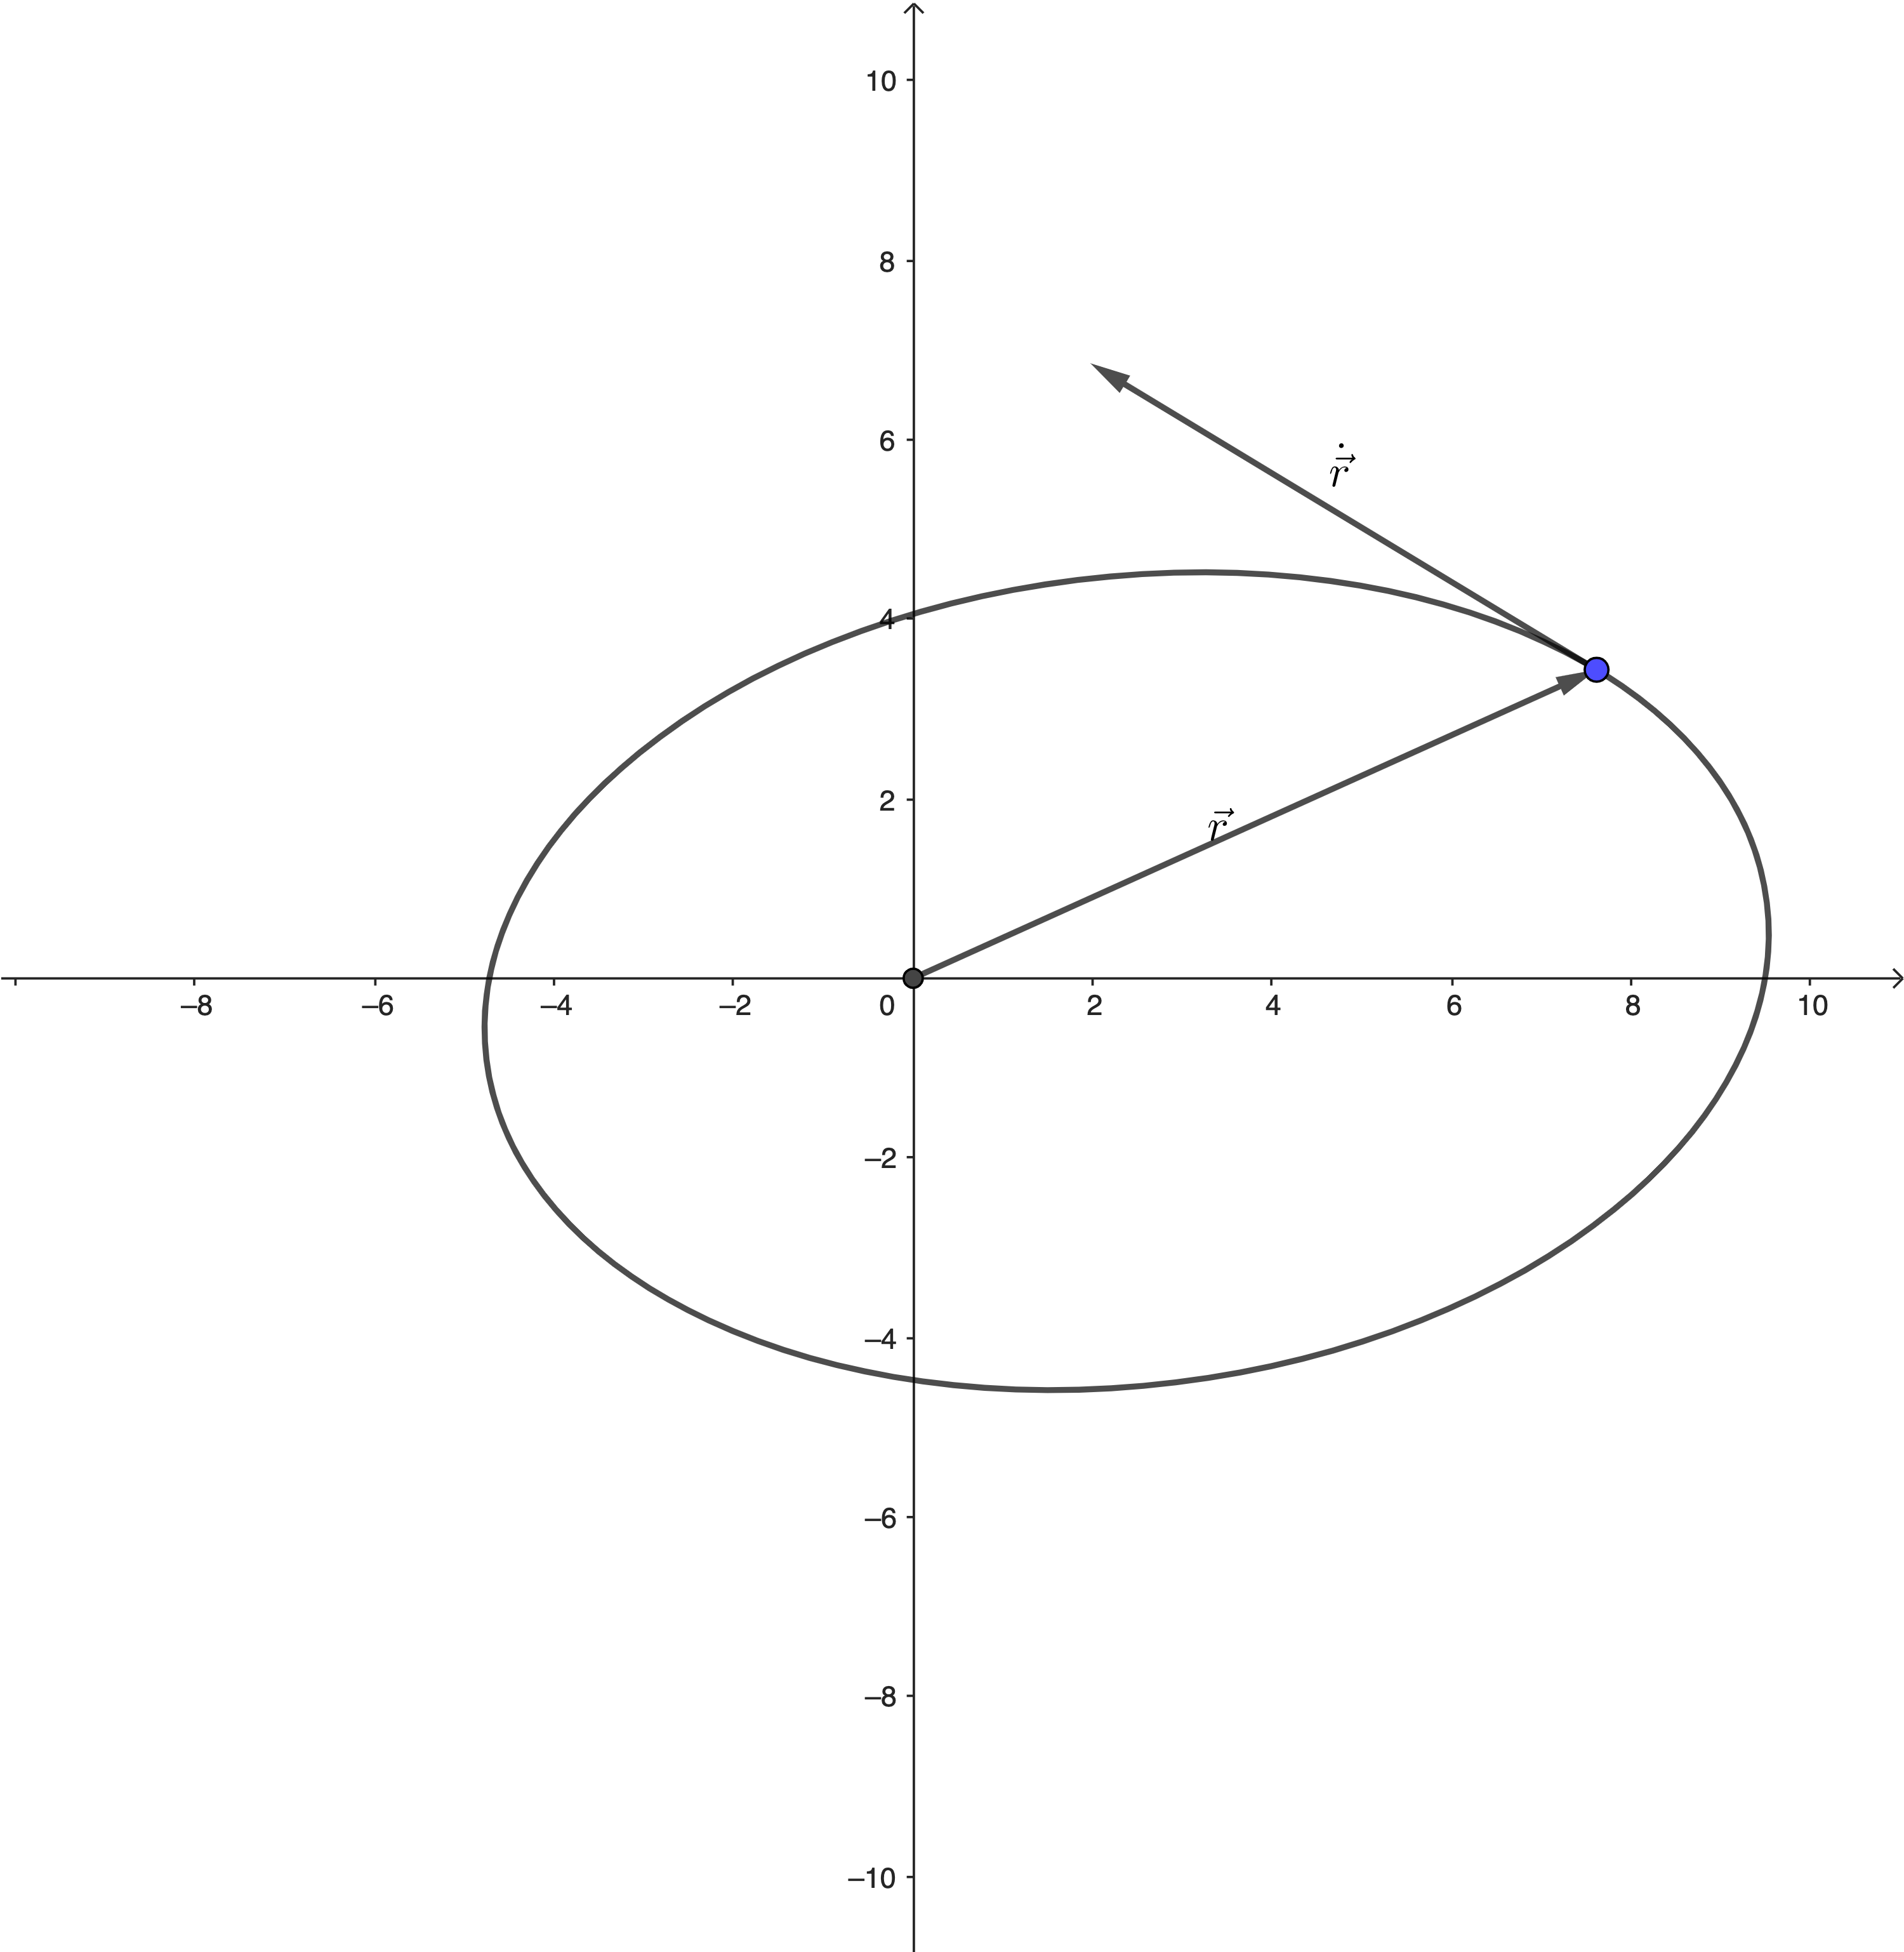
\includegraphics[width = 0.5 \textwidth]{Tangentialvektor.png}
\end{center}
\clearpage

\begin{bsp}
    {Diskussion einer Parametrisierten Kurve}{}
    Gegeben ist die parametrisierte Kurve mit der Gleichung:
    $$ \vec{r}: [0, 2\pi] \to \R^2, \quad \vec{r}(t) = \begin{pmatrix}
        1-\sin(2t) \\ 
        \cos(t)
    \end{pmatrix}$$
    Bestimme die Achsenschnittpunkte und die Kurvenpunkte mit Tangenten parallel zu den Koordinatenachsen. Skizziere anschliessend die Kurve.

    \vspace*{18 cm}

\end{bsp}

\clearpage
\begin{ueb}
    {}{}

\begin{enumerate}
    \item Kreise
    \begin{enumerate}
        \item Betrachten Sie die Parameterdarstellung eines Kreises mit Radius 1: $$\vec{r}(t) = \begin{pmatrix}
            \cos(t) \\ \sin(t)
        \end{pmatrix} , \quad t \in [0, 2\pi] $$
        Zeigen Sie mit dem Skalarprodukt, dass $\dot{\vec{r}} (t)$ und $\vec{r}(t)$ senkrecht aufeinander stehen.

        In welche Richtung zeigt $\ddot {\vec{r}}$ ?
        \item Betrachten Sie eine alternative Parametergleichung für den Kreis:
        $$\vec{r}_2(t) = \begin{pmatrix}
            \cos(2t) \\ \sin(2t)
        \end{pmatrix} , t \in [0, \pi] $$
        Vergleichen Sie $\dot{\vec{r_2}} (t)$ mit $\dot {\vec{r}} (t)$ aus Aufgabe (a). Interpretation?
    \end{enumerate}


    \item Die folgenden Kurven sind in Parameterdarstellung gegeben. Bestimmen Sie rechnerisch die Schnittpunkte mit den Koordinatenachsen und die Kurvenpunkte mit Tangenten parallel zu den Koordinatenachsen. Zeichnen Sie diese Kurven mit Geogebra und überprüfen Sie damit Ihre Lösungen.

    \begin{enumerate}
        \item \(\begin{pmatrix}
            x \\
            y
        \end{pmatrix} = \begin{pmatrix}
            t \\
            2t^2 + t - 1
        \end{pmatrix}\)
    
        \item \(\begin{pmatrix}
            x \\
            y
        \end{pmatrix} = \begin{pmatrix}
            t^2 - 1 \\
            t^3 - t
        \end{pmatrix}\)
    
        \item \(\begin{pmatrix}
            x \\
            y
        \end{pmatrix} = \begin{pmatrix}
            \sin 2t \\
            \cos t
        \end{pmatrix}\)
    
        \item \(\begin{pmatrix}
            x \\
            y
        \end{pmatrix} = \begin{pmatrix}
            2\sqrt{2 + t} \\
            \sqrt{2 - t}
        \end{pmatrix}\)
    
        \item \(\begin{pmatrix}
            x \\
            y
        \end{pmatrix} = \begin{pmatrix}
            t - \sin t \\
            1 - \cos t
        \end{pmatrix}\)
    
        \item \(\begin{pmatrix}
            x \\
            y
        \end{pmatrix} = \begin{pmatrix}
            1 + \sin t \\
            2 \cos 2t
        \end{pmatrix}\)
    
        % \item \(\begin{pmatrix}
        %     x \\
        %     y
        % \end{pmatrix} = \begin{pmatrix}
        %     t - \sin t \\
        %     t - \cos t
        % \end{pmatrix}\)
    
        \item \(\begin{pmatrix}
            x \\
            y
        \end{pmatrix} = \begin{pmatrix}
            \sinh t \\
            \cosh t
        \end{pmatrix} = \frac{1}{2}\begin{pmatrix}
            e^t - e^{-t} \\ 
            e^t + e^{-t}
        \end{pmatrix}\)
    \end{enumerate}
\end{enumerate}
    
\end{ueb}

\clearpage
\emph{Lösungen}
\begin{enumerate}
    \item Easy :) 
    \item 
\begin{enumerate}
    \item Parabel:
    
    Achsenschnittpunkte $ \left(-1, 0\right), \left(\frac{1}{2}, 0\right), \left(0, -1\right)$. 
    
    Tangenten parallel zur $x$-Achse: $ \left(-\frac{1}{4}, -\frac{9}{8}\right)$. 

    Tangenten parallel zur $y$-Achse: Keine.

    \item ``Parabola nodata''
    
    Achsenschnittpunkte $ \left(-1, 0\right), \left(0, 0\right)$. 
    
    Tangenten parallel zur $x$-Achse: $ \left(-\frac{2}{3}, \pm\frac{2\sqrt{3}}{9}\right)$. 

    Tangenten parallel zur $y$-Achse: $\left(-1, 0\right)$


    \item Achsenschnittpunkte $ \left(0, 0\right), \left(0, \pm 1\right)$. 
    
    Tangenten parallel zur $x$-Achse: $ \left(0, \pm 1\right)$. 

    Tangenten parallel zur $y$-Achse: $\left(\pm1, \pm\frac{\sqrt{2}}{2}\right)$

    \item Achsenschnittpunkte $ \left(4, 0\right), \left(0, 2\right)$. 
    
    Tangenten parallel zur $x$-Achse: keine. 

    Tangenten parallel zur $y$-Achse: keine.

    \item Achsenschnittpunkte $ \left(2k\pi, 0\right)$. 
    
    Tangenten parallel zur $x$-Achse:  $ \left((2k+1)\pi, 2\right)$. 

    Tangenten parallel zur $y$-Achse: keine.
    
    \item ``Zykloide''
    
    Achsenschnittpunkte $ \left(1\pm\frac{\sqrt{2}}{2}, 0\right), \left(0, -2\right)$. 
    
    Tangenten parallel zur $x$-Achse: $ \left(1, 2\right)$. 

    Tangenten parallel zur $y$-Achse: keine.

    \item Hyperbel
    
    Achsenschnittpunkte $ \left(0, 1\right)$. 
    
    Tangenten parallel zur $x$-Achse: $ \left(0, 1\right)$.

    Tangenten parallel zur $y$-Achse: keine.



    
\end{enumerate}
\end{enumerate}





\clearpage
\section{Die Bogenlänge parametrisierter Kurven}
Die Einführung zu diesem Kapitel wird im Unterricht behandelt\dots


% Durchläuft man eine Kurve, so legt man dabei eine gewisse Distanz zurück. Aber wie berechnet man die Länge des zurückgelegten Weges?

% Rufen wir uns dazu in Erinnerung, dass die Momentangeschwindigkeit $\vec{v}(t)$ der parametrisierten Kurve $\vec{r}(t)$ zum Zeitpunkt $t$ dem Tangentialvektor $\vec{v}(t) = \dot{\vec{r}}(t)$ entspricht. So ist intuitiv klar, dass der zurückgelegte Weg zwischen den Zeitpunkten $a$ und $b$ durch das Integral der Schnelligkeit $|\dot{\vec{r}}(t)|$ über dem Intervall $[a, b]$ gegeben ist.

\begin{definition}
    {Bogenlänge einer Kurve}{Bogenlänge}
    Sei $\vec{r}: \, [a,b] \longrightarrow \mathbb{R}^n$ eine parametrisierte Kurve. Dann heisst
    $$L \; = \; \int\limits_{a}^{b} \, |\dot{\vec{r}}(t)| \, dt $$
    die Bogenlänge von $\vec{r}(t)$.
\end{definition}

\begin{bsp}{Bogenlänge eines Halbkreises}{}
    Der Halbkreis vom Radius $R$ in der oberen Halbebene des $\mathbb{R}^2$ mit Zentrum im Ursprung lässt sich auf ganz unterschiedliche Weisen parametrisieren. Wir betrachten hier die beiden Parametrisierungen
    $$\vec{r}_1:[0,1] \longrightarrow \mathbb{R}^2, \;\;\; \vec{r}_1(t) = \begin{pmatrix}
    R \, \cos (\pi \, t) \\ 
    R \, \sin(\pi \, t)
    \end{pmatrix} $$
    %\hspace{0.3cm} \mbox{sowie} \hspace{0.3cm}
   
    \vspace*{12cm}
    \pagebreak
    $$ \vec{r}_2:[0,\pi \, R] \longrightarrow \mathbb{R}^2, \;\;\; \vec{r}_2(t) = \begin{pmatrix}
    R \, \cos (t/R) \\ 
    R \, \sin(t/R)
    \end{pmatrix}$$

    \vspace*{10cm}
\end{bsp}

\begin{bsp}
    {Bogenlänge einer Schraubenlinie}{}
    Betrachten wir die Raumkurve $\vec{r}:\mathbb{R} \longrightarrow \mathbb{R}^3$, $\vec{r}(t) = \begin{pmatrix} 3\cos(t) \\ 3\sin(t) \\ 4t \end{pmatrix}$.
    \begin{center}
        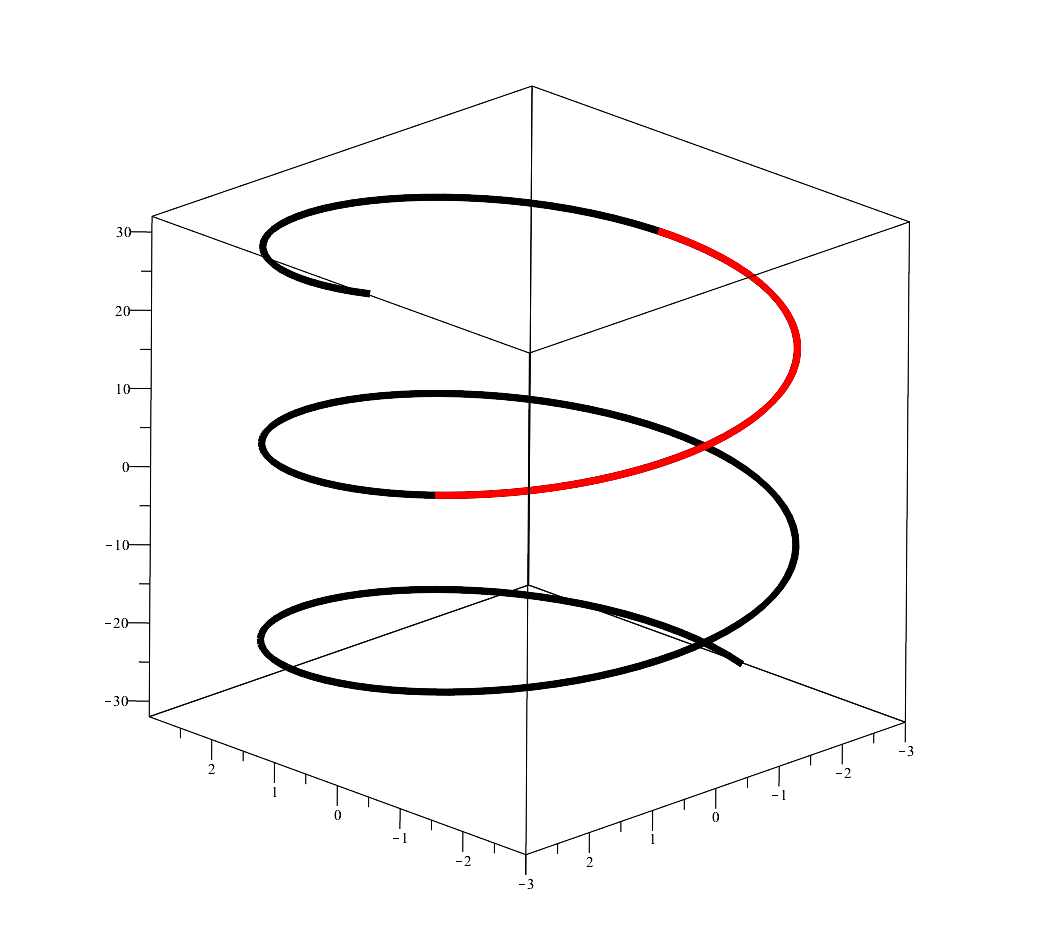
\includegraphics[width=0.5\textwidth]{spiral.png} 
    \end{center}
    Ihre Spur ist eine unendliche Schraubenlinie um die $z$-Achse. Im folgenden soll die Bogenlänge des rot markierten Kurvenstücks berechnet werden. Dieses entspricht dem Teil der Bahn, der zwischen den Zeitpunkten $t_1=0$ und $t_2=2$ durchlaufen wird.
    
\vspace*{10cm}
% Ihre Spur ist eine unendliche Schraubenlinie um die $z$-Achse. Die Momentangeschwindigkeit $\vec{v}(t)$ zum Zeitpunkt $t$
% ist durch $\vec{v}(t) = \dot{\vec{r}}(t) = \begin{pmatrix} -3\sin(t) \\ 3\cos(t) \\ 4 \end{pmatrix}$ gegeben. Ihr Betrag berechnet sich vermöge der trigonometrischen Identität 
% $$\sin^2(t) + \cos^2(t) = 1$$ 
% zu $|\dot{\vec{r}}(t)| = 5$. Daraus folgt, dass die Kurve über dem Parameterintervall $[t_0, t_1] = [0, 2]$ eine Länge von
% $$ L[\, \vec{r} \, _{[0,2]}] = \int\limits_{0}^{2} |\dot{\vec{r}}(t)| \, dt
% = \int\limits_{0}^{2} 5 \, dt
% = \Big[ 5t \Big]_{0}^{2} = 10$$
% besitzt.



\end{bsp}
\pagebreak
\begin{ueb}
{}{}
\begin{enumerate}
    \item Skizzieren Sie die Spuren der folgenden Kurven (Geogebra) und berechnen Sie ihre Bogenlängen:

    \begin{enumerate}
    \item $\vec{r}: [0,\pi] \rightarrow \mathbb{R}^2$, \quad $\vec{r}(t) = \begin{pmatrix} 3 \cdot \cos(t) \\ 3 \cdot \sin(t) \end{pmatrix}$
    \item $\vec{r}: [-1,1] \rightarrow \mathbb{R}^2$, \quad $\vec{r}(t) = \begin{pmatrix} t \\ t^2 \end{pmatrix}$ (Integral numerisch mit dem Taschenrechner berechnen)
    \item $\vec{r}: \left[-\frac{1}{2}, \frac{1}{2}\right] \rightarrow \mathbb{R}^2$, \quad $\vec{r}(t) = \begin{pmatrix} 2t \\ 4t^2 \end{pmatrix}$ (Integral numerisch mit dem Taschenrechner berechnen)
    \item $\vec{r}: [0, 2\pi] \rightarrow \mathbb{R}^2$, \quad $\vec{r}(t) = \begin{pmatrix} \cos(t) \\ \sin(t) \\ t \end{pmatrix}$
    \item $\vec{r}: [0, 2\pi] \rightarrow \mathbb{R}^2$, \quad $\vec{r}(t) = \begin{pmatrix} t- \sin(t) \\ 1-\cos(t) \end{pmatrix}$ (Integral numerisch mit dem Taschenrechner berechnen)
    \end{enumerate}

    \item Ein Ball wird auf einer Abwurfhöhe von \SI{1.60}{\meter} mit einer Anfangsgeschwindigkeit von \SI{12}{\meter\per\second} unter einem Winkel von \SI{30}{\degree} zur Horizontalen abgeworfen. Seine Flugbahn hat dann die Parametergleichung
    \[
        \vec{r}(t) = \begin{pmatrix}
        6\sqrt{3}t \\
        6t - \frac{1}{2} g t^2 + 1.6
        \end{pmatrix}.
    \]
    
    \begin{enumerate}
        \item Berechnen Sie den Geschwindigkeitsvektor zur Zeit $t=0$ und den Beschleunigungsvektor und überprüfen Sie, ob diese zu den Angaben im Text passen.
        \item Berechnen Sie, wie lange es dauert, bis der Ball wieder auf den Boden prallt, und die (Bogen)-Länge der Flugbahn. (Integral numerisch mit dem Taschenrechner berechnen)
    \end{enumerate}


    \item Das Integral, mit dem man die Bogenlänge berechnet, ist ein Spezialfall der skalaren Kurvenintegrale (oder Kurvenintegrale 1. Art). Schauen Sie sich die beiden Videos dazu an, die im Moodle-Kurs verlinkt sind, und berechnen Sie das folgende Integral
    $$ \oint_K f\, ds$$
    wobei $K$ der Einheitskreis und $f$ die Funktion $f(x,y)=5x^2+5y^2$ ist. 

    \item Die Masse \( m \) eines Drahtes soll in Abhängigkeit eines Parameters \( \lambda \) berechnet werden. Dabei ist die ortsabhängige Dichte \( \rho \) durch die Funktion 
    \[ \rho(x,y,z) = \lambda(x + z) \] 
    gegeben.
    
    Der Draht folgt dabei der Kurve \( \mathcal{C} \) mit:
    \[
    \mathcal{C} : \, \vec{r}(t) = \begin{pmatrix} 
        \frac{2}{3}t^3\\
        t^2 \\
        t+1
    \end{pmatrix}, \quad 0 \leq t \leq 1
    \]
    
\end{enumerate}

\end{ueb}
\clearpage
\emph{Lösungen:}
\begin{enumerate}
    \item Bogenlängen berechnen
    \begin{enumerate}
        \item Halbkreis mit Radius 3: Bogenlänge $L=3\pi$.
        \item Normalparabel. Bogenlänge $L\approx 2.958$ (Das bestimmen der Stammfunktion ist in diesem Fall nicht einfach...)
        \item Es ist die gleiche Kurve wie bei (b) bloss anders parametrisiert: Bogenlänge $L\approx 2.958$ (Das bestimmen der Stammfunktion ist in diesem Fall nicht einfach...)
        \item Schraubenlinie. $L=2\sqrt{2}\pi$
        \item Zykloide. $L=8$
    \end{enumerate}
    \item Ball
    \begin{enumerate}
        \item es ist: 
        \[
            {\vec{v}(t)} = \begin{pmatrix}
            6\sqrt{3} \\
            6 - gt
            \end{pmatrix}
            \Rightarrow
            \vec{v}(0) = \begin{pmatrix}
                6\sqrt{3} \\
                6 
                \end{pmatrix}
            =
            12\begin{pmatrix}
                \frac{\sqrt{3}}{2} \\
                \frac{1}{2}
                \end{pmatrix}
            =
            12\begin{pmatrix}
                \cos(\SI{30}{\degree}) \\
                \sin(\SI{30}{\degree})
                \end{pmatrix}
        \]
        Das passt!

        Und für die Beschleunigung:
        \[
            {\vec{a}(t)} = \begin{pmatrix}
            0 \\
            - g
            \end{pmatrix}
        \]
        Das passt auch!
        \item Aufprallzeitpunkt: $y=0 \Rightarrow t \approx 1.45$ (negative Lösung ergibt im Kontext keinen Sinn)
        
        Länge der Flugbahn: $L\approx 16.23$
        
    \end{enumerate}
    \item Kurvenintegral erster Art:  $$ \oint_K f\, ds = 10\pi $$
    \item Integriere die Dichtefunktion entlang der Kurve:
    $$m = \int_C \rho \, ds = \int_0^1 \rho(r(t)) \cdot  |\dot{\vec{r}}(t)| \, dt = \frac{55}{18}\lambda$$
\end{enumerate}
\clearpage
\section{Arbeitsintegrale}
\subsection{Arbeit als Skalarprodukt}
Physikalische Grössen mit einer Richtung wie Kraft oder Geschwindigkeit werden mit Vektoren beschrieben. Bei anderen Grössen wie Temperatur, Masse oder Arbeit handelt es sich jedoch um sogenannte Skalare grössen - also um solche, die mit einer Zahl beschrieben werden. Die Verbindung zwischen vektoriellen und skalaren Grössen geschieht häufig mit dem Skalarprodukt von Vektoren.

\begin{bsp}
    {Arbeit als Skalarprodukt}{intro-Arbeit}
    Wenn unter Wirkung einer Kraft einen Weg zurückgelegt wird, wird mechanische Arbeit verrichtet. Betrachten Sie beispielsweise einen Wagen, der sich auf einer Schiene befindet und auf den seitwärts eine konstante Kraft $F$ wirkt

    \begin{center}
        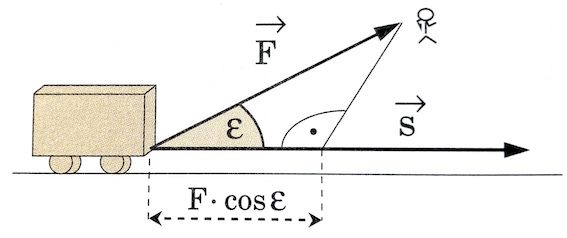
\includegraphics[width = 0.5\textwidth]{skalarprodArbeit.jpg}
    \end{center}

    

    Die Arbeit $W$ ist in diesem Fall das Produkt aus dem zurückgelegten Weg $s$ und der \emph{Komponente der Kraft längs der Schiene}:
    $$ W = \lvert\vec{F}\rvert  \cdot \cos(\varepsilon) \cdot s$$

    Die Kraftkomponente, die parallel zur Schiene verläuft, wird häufig mit dem Skalarprodukt berechnet. Wir erinnern uns an die Definition des Skalarprodukts:
    $$\langle \vec{a} , \vec{b} \rangle = \lvert\vec{a}\rvert\cdot \lvert\vec{b}\rvert \cdot \cos(\varepsilon)$$
    Somit gilt
    $$ \lvert\vec{F}\rvert  \cdot \cos(\varepsilon) = \left\langle\vec{F},  \vec{s}\right \rangle \cdot \frac{1}{\lvert\vec{s}\rvert} = \left\langle \vec{F} , \frac{\vec{s}}{\lvert\vec{s}\rvert} \right \rangle$$
    Die mechanische Arbeit, die bei der Bewegung des Wagens auf der Schiene verrichtet wird, kann schliesslich so berechnet werden:
    $$W = \left\langle\vec{F} , \frac{\vec{s}}{\lvert\vec{s}\rvert}\right\rangle \cdot s $$
    Das scheint auf den ersten Blick komplizierter als die erste Formel zu sein, diese Darstellung lässt sich jedoch gut auf die Situation übertragen, wenn die Bewegung entlang einer Kurve geschieht.

\end{bsp}

\clearpage

% In der letzten Formel im \Cref*{bsp:intro-Arbeit} oben, haben die beiden darin vorkommenden ``$\cdot$''-Zeichen zwei unterschiedliche Bedeutungen. Das erste $\cdot$ innerhalb der Klammern steht für das Skalarprodukt von zwei Vektoren. Das zweite hingegen für die Multiplikation von zwei reellen Zahlen. Damit es nicht zu Verwechslungen kommt – insbesondere auch darum, weil wir teilweise auf die Vektorpfeile verzichten – führen wir für das Skalarprodukt die Notation ein, die auch an Hochschulen verwendet wird: 

% \begin{definition}
%     {Schreibweise für das Skalarprodukt}{}
%     Seien $\vec{a}$ und $\vec{b}$ zwei Vektoren. Dann schreiben wir für das Skalarprodukt der beiden Vektoren
%     $$\langle \vec{a}, \vec{b} \rangle $$

% \end{definition}

% Mit dieser Schreibweise lautet die Formel für die mechanische Arbeit aus  \Cref*{bsp:intro-Arbeit}:
% $$W = \langle \vec{F}, \frac{\vec{s}}{\lvert\vec{s}\rvert}\rangle \cdot s $$


\subsection{Arbeit entlang eines Weges in einem Kraftfeld}
Im Folgenden soll die Situation mit dem Wagen aus \Cref*{bsp:intro-Arbeit} auf zwei Arten verallgemeinert werden: Die wirkende Kraft $\vec{F}$  soll nicht mehr konstant sein und die Bewegung soll nicht mehr entlang einer Geraden stattfinden.

\emph{Aus der Kraft wird ein Kraftfeld}

Beginnen wir damit, dass die Kraft nicht mehr konstant ist. Damit ist gemeint, dass die wirkende Kraft abhängig ist vom Ort, an dem sich das Objekt befinden. In anderen Worten: Jedem Ort in wird eine Kraft zugeordnet. Das ist eine Funktion!
\begin{definition}
    {Vektorfelder}{vektorfeld}
    Ein Vektorfeld ist eine Funktion, die jedem Punkt in der Ebene (oder im Raum) einen Vektor zuordnet.

    Ein Vektorfeld ist somit eine Abbildung der Form:
    $$ \vec{V} : \R^2 \to \R^2$$
\end{definition}
Vektorfelder stellt man sich am besten so vor: Jedem Punkt der Ebene wird ein Vektor zugeordnet, der von diesem Punkt aus startet.

\begin{center}
\begin{tikzpicture}[scale = 0.3]
    \foreach \x in {-10,-9,...,10}
        \foreach \y in {-10,-9,...,10}
            \draw[->, blue] (\x,\y) -- (\x-\y/10,\y+\x/10);

    % Achsen
    \draw[thick,->] (-11,0) -- (11,0) node[right] {$x$};
    \draw[thick,->] (0,-11) -- (0,11) node[above] {$y$};
    
    % Gitterlinien
    \foreach \x in {-10,-9,...,10}
        \draw[thin, gray, dashed] (\x,-10) -- (\x,10);
    \foreach \y in {-10,-9,...,10}
        \draw[thin, gray, dashed] (-10,\y) -- (10,\y);
\end{tikzpicture}
\end{center}

Die physikalische Bedeutung solcher Vektorfelder kann ganz unterschiedlich sein. Wir werden Sie häufig als Kraftfelder betrachten. Der Bildvektor ist dann die an der betrachteten Position wirkende Kraft. Mit Vektorfelder kann aber zum Beispiel auch die Strömung einer Flüssigkeit beschrieben werden. In diesem Fall steht der Bildvektor für die Geschwindigkeit der Flüssigkeit an der betrachteten Stelle.

\clearpage

\emph{Aus der geraden Schiene wird eine Kurve}

Wir kommen nun zur zweiten Verallgemeinerung des \Cref*{bsp:intro-Arbeit}. Anders als im Beispiel soll die Bewegung entlang einer Kurve stattfinden, von der die Parametrisierung gegeben ist: $$\vec{r}: [a,b]\to\R^2,\quad  t\mapsto \vec{r}(t)$$

\begin{center}
    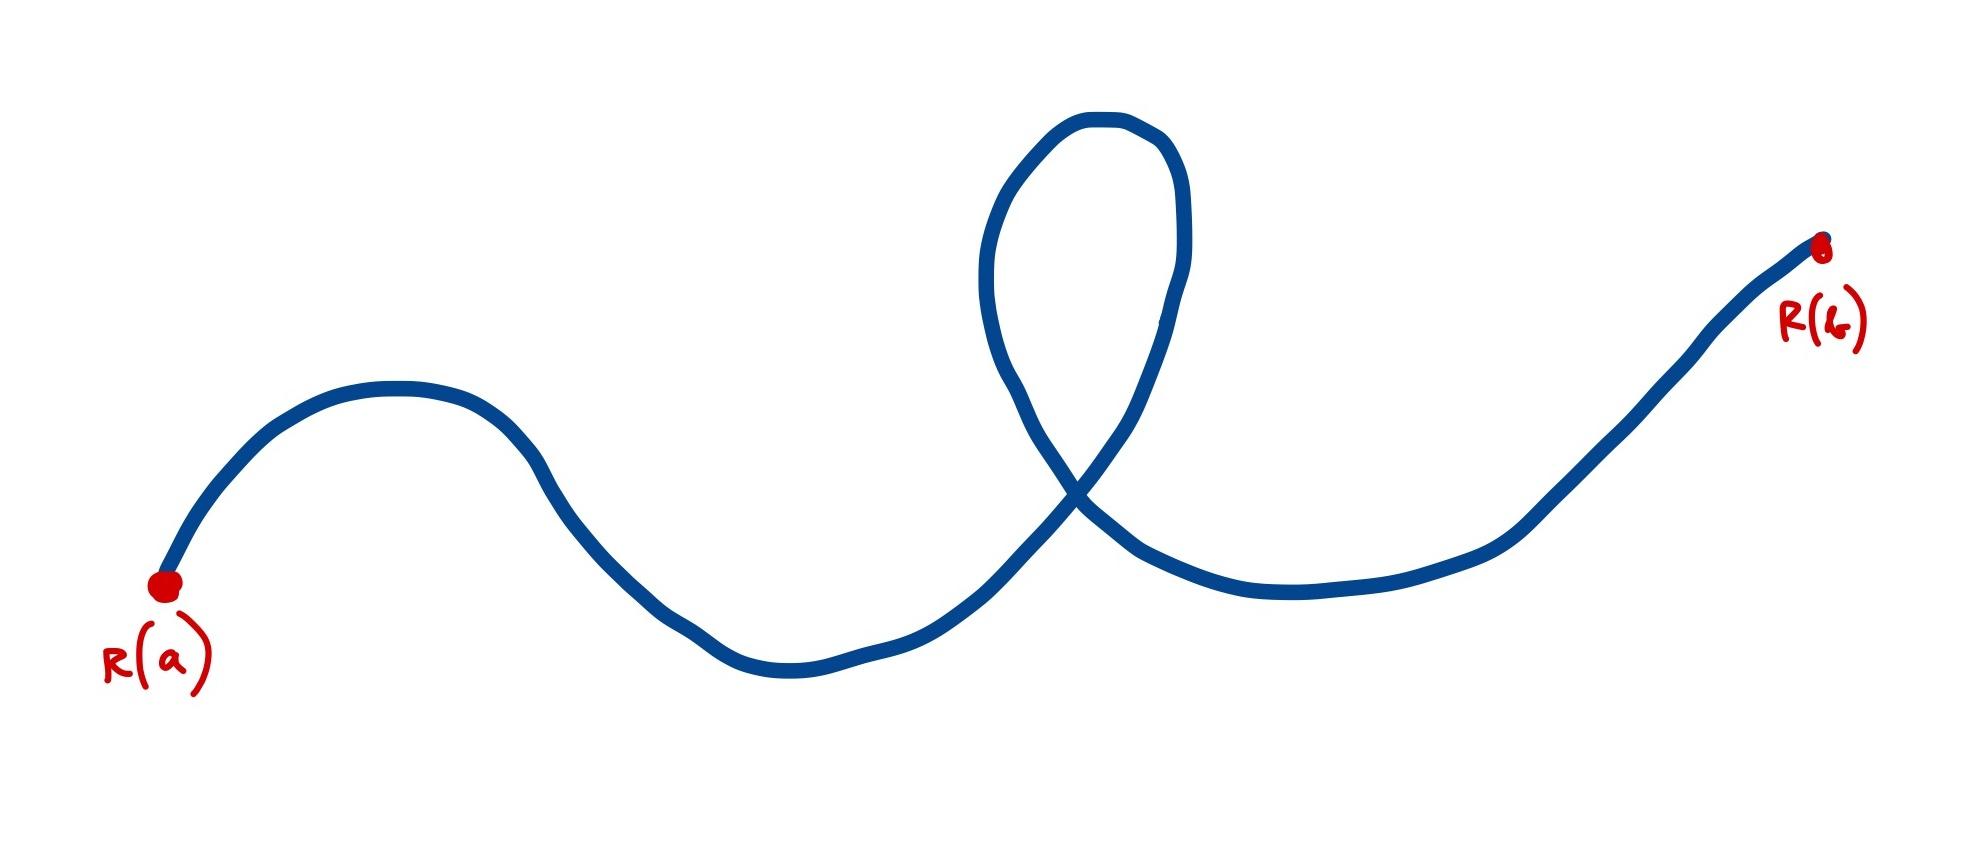
\includegraphics[width = 0.7\textwidth]{ArbeitsintegralSkizze1.jpg}
\end{center}

Um die verrichtete Arbeit näherungsweise zu bestimmen, wird das Intervall $[a,b]$ in $n$ kleine Teilintervalle mit den Grenzen $a=t_0, t_1, t_2, \dots, t_n = b$ unterteilt. Die entsprechenden Kurvenstücke sind dann nahezu gerade. Damit kann die Arbeit für ein solches Kurvenstück mit der Formel $W = \left\langle \vec{F}, \frac{\vec{s}}{\lvert\vec{s}\rvert}\right\rangle \cdot s$ für die Arbeit entlang einer Geraden approximiert werden.  Für die verrichtete Arbeit $W_k$ im Zeitintervall $[t_k, t_{k+1}]$ gilt: 
$$W_k \approx \left\langle \vec{F}(\vec{r}(t_k)), \frac{\dot{\vec{r}}(t_k)}{\lvert\dot{\vec{r}}(t_k)\rvert} \right\rangle \cdot \Delta s$$

\begin{center}
    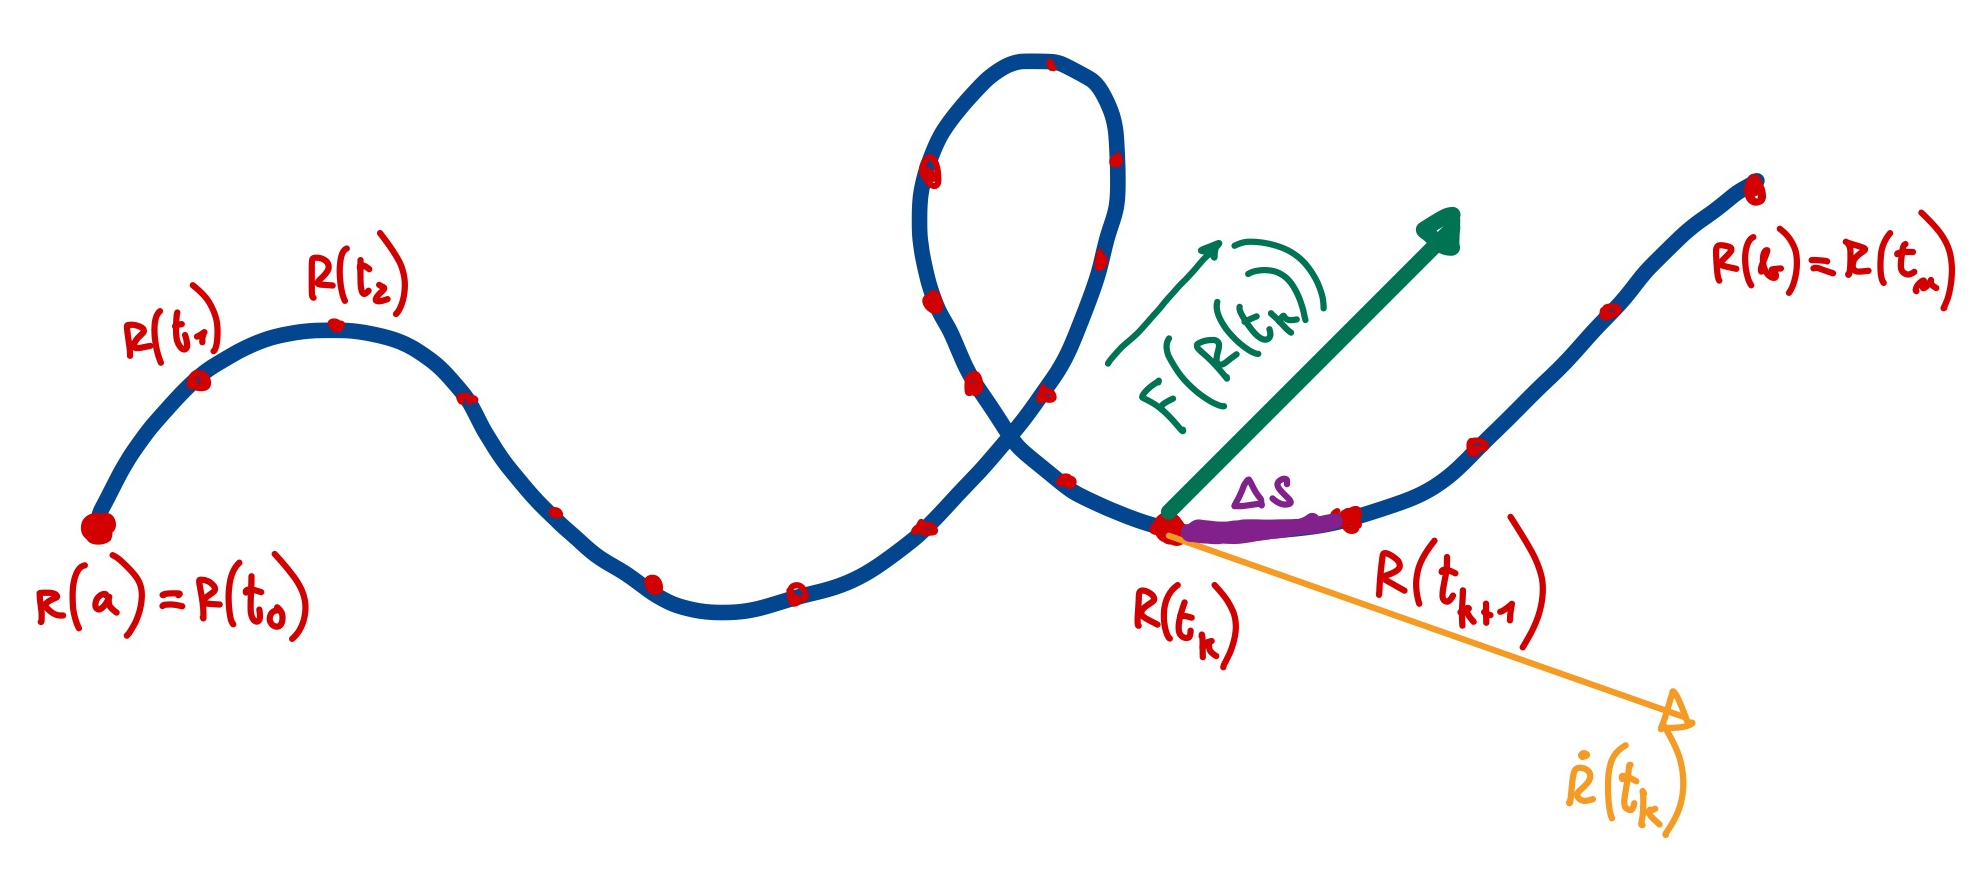
\includegraphics[width = 0.7\textwidth]{ArbeitsintegralSkizze2V2.png}
\end{center}

Diese Formel kann etwas vereinfacht werden, wenn man berücksichtigt, dass der im Intervall $[t_k, t_{k+1}]$ zurückgelegte Weg $\Delta s$ aus der Schnelligkeit $|\dot{\vec{r}}(t_k)|$ und der verstrichenen Zeit $\Delta t = t_{k+1} - t_k$ berechnet werden kann: $\Delta s = |\dot{\vec{r}}(t_k)|\cdot \Delta t$. Somit folgt:

$$W_k \approx \left\langle \vec{F}(\vec{r}(t_k)), \frac{\dot{\vec{r}}(t_k)}{\lvert\dot{\vec{r}}(t_k)\rvert} \right\rangle \cdot |\dot{\vec{r}}(t_k)|\cdot \Delta t = \left\langle \vec{F}(\vec{r}(t_k)), \dot{\vec{r}}(t_k) \right\rangle \cdot \Delta t $$


Für die gesamte Arbeit gilt dann:
$$W \approx \sum_{k=0}^{n} \left\langle \vec{F}(\vec{r}(t_k)), \dot{\vec{r}}(t_k) \right\rangle \cdot \Delta t$$
Diese Approximation wird umso besser, je mehr und je kleiner die Teilintervalle sind. Für $n\to\infty$ erhält man schliesslich:
$$ W = \int_{a}^{b} \left\langle \vec{F}(\vec{r}(t)), \dot{\vec{r}}(t) \right\rangle  \,  dt$$

\begin{definition}
    {Arbeitsintegrale}{Arbeitsintegral oder Wegintegrale 2. Art}
    Sei $\vec{F}: \R^2\to\R^2$ ein Vektorfeld und $\vec{r}: [a,b]\to\R^2, \, t\mapsto \vec{r}(t)$ eine parametrisierte Kurve. Dann ist das Arbeitsintegral von $\vec{F}$ entlang der Kurve $\vec{r}$ definiert als
    $$ W = \int_{a}^{b} \left\langle \vec{F}\left(\vec{r}(t)\right), \dot{\vec{r}}(t) \right\rangle  \,  dt$$
    Man schreibt dafür kurz
    $$W =\int_{\vec{r}} \vec{F} \, d\vec{s}$$
\end{definition}

\begin{bsp}{Arbeitsintegral im Wirbelfeld}{Wirbelfeld2Wege}
    Gegeben ist das Vektorfeld $\vec{F}(x,y) = \begin{pmatrix}
        -y \\x
    \end{pmatrix}$ und die Kurven $\vec{r}_1 : [0,1]\to \R^2, \,  t \mapsto \begin{pmatrix}
        1-2t \\ 0
    \end{pmatrix}  $ und $\vec{r}_2 : [0, \pi]\to \R^2, \,  t \mapsto \begin{pmatrix}
        \cos t \\ \sin t
    \end{pmatrix}  $
    
    Gesucht sind die beiden Arbeitsintegrale  $\int_{\vec{r}_1} \vec{F} \, d\vec{s}$ und $\int_{\vec{r}_2} \vec{F} \, d\vec{s}$
    \vspace*{5cm}

    \pagebreak
    \phantom{2}

    \vspace*{12cm}
\end{bsp}


\begin{ueb}
    {}{}
    Ein Kraftfeld $\vec{F}:\mathbb{R}^3\longrightarrow \mathbb{R}^3$ sei durch
$$\vec{F} : \, (x,y,z) \; \longmapsto \; 
\left( \begin{array}{c}
x \\
yz \\
z^2-x
\end{array}\right) $$
gegeben. 


Berechnen Sie die Arbeit, die verrichtet wird, wenn ein Massenpunkt entlang der parametrisierten Wege $\vec{c}_1$ bzw. $\vec{c}_2$ verschoben wird, wobei die beiden Kurven $\vec{c}_{1,2}:[0,1]\longrightarrow \mathbb{R}^3$, gegeben sind durch
$$\vec{c}_1(t) \; = \; \left( \begin{array}{c}
t \\
1-t \\
t
\end{array}\right) 
\hspace{1cm} \mbox{bzw.} \hspace{1cm}
\vec{c}_2(t) \; = \; \left( \begin{array}{c}
t^2 \\
1-t \\
t
\end{array}\right) $$
und beide die Punkte $A=(0,1,0)$ und $B=(1,0,1)$ miteinander verbinden.
\end{ueb}

\emph{Lösung:} $W_1 = \frac{1}{6}, \quad W_2 = \frac{1}{3}$










\clearpage
\section{Gradientenfelder und Potentiale}
\begin{LA}{Einführung}{ArbeitOszillator2D}
    Betrachten wir einen Massenpunkt, der im Ursprung unseres Koordinatensystems so gelagert ist, dass seine Auslenkung in Richtung der Koordinatenachsen, etwa durch zwei Federn realisiert, eine Rückstellkraft proportional zur Auslenkung erfährt, die in  \(y\)-Richtung doppelt so gross sei, wie in \(x\)-Richtung.
    \begin{center}
        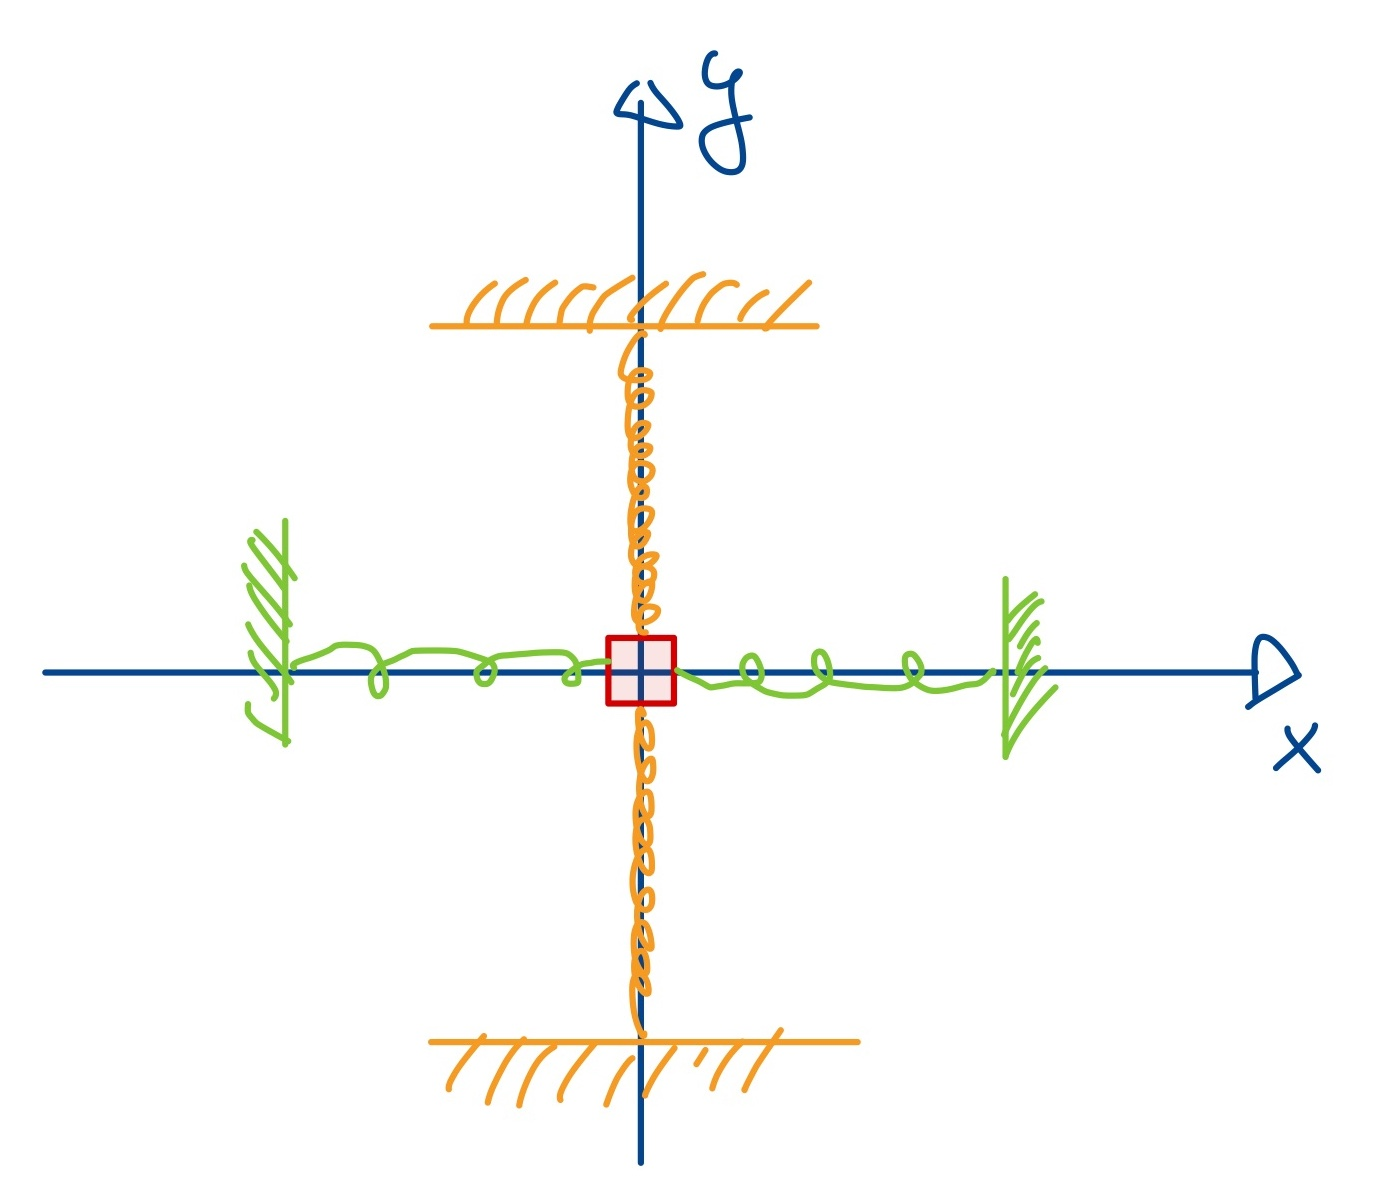
\includegraphics[width=0.5\textwidth]{harmosz2d.jpg}
    \end{center}
    Das wirkende Kraftfeld ist dann \(\vec{F}(x,y)=\begin{pmatrix}
        -x \\ -2y
    \end{pmatrix}\).

    Der Massenpunkt soll nun von der Ruhelage zum Punkt \((-2, 0)\) bewegt werden. Einmal entlang der geraden Verbindung \(\vec{r}_1 : [0,2] \to \R^2, t \mapsto \begin{pmatrix}
        -t \\ 0
    \end{pmatrix}\) und einmal entlang des Halbkreises \(\vec{r}_2 : [0,\pi] \to \R^2, t \mapsto \begin{pmatrix}
        \cos(t) - 1 \\ \sin(t)
    \end{pmatrix}\)

    Berechnen Sie für jeden Weg die verrichtete Arbeit und vergleichen Sie die Resultate.
    (Zur Vereinfachung des Integranden beim Halbkreisweg kann die Doppelwinkelformel helfen: \(\sin(2x) = 2 \sin(x)\cos(x)\) woraus folgt: \(\sin(x)\cos(x)) = \frac{1}{2} \sin(2x)\)


\end{LA}
\clearpage
Im Einführungsbeispiel wird für beide Wege von \((0,0)\) zum Punkt \((-2,0)\) die gleiche Arbeit verrichtet. Das ist kein Zufall!

\begin{satz}
    {Wegunabhängigkeit eines Arbeitsintegrals}{}
    Sei \(\vec{F}: \R^2 \to \R^2\) ein (stetiges) Vektorfeld. Falls es eine Funktion \(\Phi : \R^2 \to \R\) gibt, mit der Eigenschaft \(\vec{\nabla} \Phi = \vec{F}\), dann ist der Wert eines Arbeitsintegrals entlang einer Kurve \(K\) nur von deren Anfangspunkt \(A\) und dem Endpunkt \(B\) abhängig.
    Genauer gilt:

    \[ \int_K \vec{F} d\vec{s} = \Phi(B) - \Phi(A)\]
\end{satz}

Diese Aussage ist quasi die höherdimensionale Entsprechung des Hauptsatzes der Differential- und Integralrechnung aus dem Grundlagefach: \(\int_{a}^{b} f(x) dx = F(b) - F(a)\)


\begin{definition}
    {Gradientenfeld, konservatives Vektorfeld, Potential}{}
    Ein Vektorfeld \(\vec{F}\) mit der Eigenschaft \(\vec{\nabla} \Phi = \vec{F}\) nennt man ein Gradientenfeld oder ein konservatives Vektorfeld.

    Die Funktion \(\Phi\) nennt man das zugehörige (Skalar-)Potential.
\end{definition}
\begin{bsp}
    {Potential des zweidimensionalen Oszillators}{
    }
    Betrachten wir noch einmal das Kraftfeld aus \Cref*{LA:ArbeitOszillator2D}: \(\vec{F}(x,y)=\begin{pmatrix}
        -x \\ -2y
    \end{pmatrix}\).

    Man kann leicht einsehen, dass \(\vec{F}\) das Gradientenfeld des Potentials \(\Phi(x,y) = -\frac{1}{2} x^2 - y^2\) ist.

    Für die beiden Wege \(\vec{r}_1\) und \(\vec{r}_2\) aus \Cref*{LA:ArbeitOszillator2D}, welche die beiden Punkte \(A=(0,0)\) und \(B=(-2,0)\) verbinden, gilt dann:
    \[\int_{\vec{r}_1} \vec{F} d\vec{s} =\int_{\vec{r}_2} \vec{F} d\vec{s} = \Phi(-2,0) - \Phi(0,0) = -\frac{1}{2} (-2)^2 = -2\]

\end{bsp}

Das Beispiel gibt auch eine physikalische Interpretation des Potentials. Mit der Funktion \(\Phi\) im Beispiel des zweidimensionalen Oszillators lässt sich die potentielle Energie (im Fall der Feder heisst das Spannenergie) des Massenpunkts berechnen. Es gilt nämlich: Die Spannenergie eines Massenpunktes, der sich an der Stelle \((x,y)\) im Kraftfeld \(\vec{F}\) befindet, ist \(E_{\text{spann}} = - \Phi(x,y)\). Der Wert des Arbeitsintegrals ist dann die Differenz der Spannenergie am Anfangspunkt und jener am Endpunkt des Weges.\footnote{Im Kontext der Physik wird das Potential darum auch häufig als die Funktion definiert, für welche \(\vec{\nabla} \Phi = - \vec{F}\) ist.}

\begin{bsp}
    {Das Wirbelfeld ist kein Gradientenfeld}{AnsatzmethodefürPotential}
    Wir betrachten nochmals die Situation aus \Cref*{bsp:Wirbelfeld2Wege}. Wie wir dort bereits berechnet haben, gilt für das Vektorfeld \(\vec{F}(x,y) = \begin{pmatrix}
        -y \\x
    \end{pmatrix}\) und für die beiden Kurven
    \[\vec{r}_1 : [0,1]\to \R^2, t \mapsto \begin{pmatrix}
            1-2t \\ 0
        \end{pmatrix}  \quad \text{und}\quad  \vec{r}_2 : [0, \pi]\to \R^2, t \mapsto \begin{pmatrix}
            \cos t \\ \sin t
        \end{pmatrix}  \]
    dass
    \[ \int_{\vec{r}_1} \vec{F} \, d\vec{s} = 0 \, \neq \int_{\vec{r}_2} \vec{F} \, d\vec{s} = \pi\]

    Obwohl beide Kurven von \(A=(1,0)\) nach \(B=(-1,0)\) verlaufen, haben die Integrale einen unterschiedlichen Wert. Das liegt darin, dass das Vektorfeld \(\vec{F}\) kein Gradientenfeld ist. Das lässt sich leicht einsehen:

    \vspace*{15cm}

    %    Angenommen es gäbe eine Funktion $\Phi: \R^2 \to \R$ mit $\vec{\nabla}\Phi(x,y) = \vec{F}(x,y) = \begin{pmatrix}
    %     -y \\x
    %    \end{pmatrix}$. Dann müsste 
    %    $$\frac{\partial\Phi(x,y)}{\partial x} = -y$$
    %    sein. Durch Integration nach $x$ folgt:
    %    $$\Phi(x,y) = -xy + c_1 (y)$$
    %    Wobei $c_1(y)$ ein Term ist, der zwar von $y$ nicht aber von $x$ abhängig ist.

    %    Gleichzeitig muss auch
    %    $$\frac{\partial\Phi(x,y)}{\partial y} = x$$
    %    gelten. Woraus wieder durch Integration – diesmal nach $y$ – folgt:
    %    $$\Phi(x,y) = xy + c_2(x)$$
    %    Insgesamt erhält man:
    %    $$-xy + c_1 (y)=\Phi(x,y) = xy + c_2(x) \iff c_1(y)+c_2(x)=2xy$$
    %    Diese Gleichung ist offensichtlich für keine Wahl der Termen $c_1(y)$ und $c_2(x)$ erfüllbar.

\end{bsp}
Für die Berechnung von Arbeitsintegral der Form \(\int_{K} \vec{F} \, d\vec{s}\) empfiehlt sich das folgende Vorgehen:
\begin{itemize}
    \item Versuche dem \Cref*{bsp:AnsatzmethodefürPotential} folgend, ein Potential \(\Phi\) zu finden mit \(\vec{\nabla}\Phi = \vec{F}\)
    \item Wenn erfolgreich: \(\int_{K} \vec{F} \, d\vec{s} = \Phi(B)-\Phi(A)\), wobei \(A\) der Anfangs- und \(B\) der Endpunkt der Kurve ist.
    \item Wenn nicht erfolgreich (oder nicht möglich): Berechne \(\int_{K} \vec{F} \, d\vec{s} =\int_{a}^{b}\langle \vec{F}(\vec{r}(t)), \dot{r}(t) \rangle  \,  dt\)
\end{itemize}

Um zu entschieden, ob ein Vektorfeld ein Gradientenfeld ist, kann man manchmal auch die folgende Überlegung verwenden. Wir erinnern uns, dass für eine zweimal stetig differenzierbare Funktion \(\Phi: \R^2 \to \R\) die gemischten partiellen Ableitungen gleich sind, also
\begin{satz}
    {Satz von Schwarz}{
    }
    Sei \(\Phi: \R^2 \to \R\) eine zweimal stetig differenzierbare Funktion. Dann gilt:
    \[\frac{\partial^2 \Phi}{\partial x \partial y} = \frac{\partial^2 \Phi}{\partial y \partial x}\]
\end{satz}

Für ein Gradientenfeld \(\vec{F} = \begin{pmatrix}
    F_1 \\ F_2
\end{pmatrix} = \vec{\nabla} \Phi = \begin{pmatrix}
    \frac{\partial \Phi}{\partial x} \\ \frac{\partial \Phi}{\partial y}
\end{pmatrix}\) gilt also:
\[  \frac{\partial F_2}{\partial x}-\frac{\partial F_1}{\partial y} =  \frac{\partial^2 \Phi}{\partial x \partial y}-\frac{\partial^2 \Phi}{\partial y \partial x}  = 0\]

\begin{definition}
    {Rotation}{}
    Sei \(\vec{F} = \begin{pmatrix}
        F_1 \\ F_2
    \end{pmatrix}\) ein Vektorfeld. Dann nennt man den Ausdruck
    \[\text{rot}(\vec{F}) = \frac{\partial F_2}{\partial x} - \frac{\partial F_1}{\partial y}\]
    die Rotation von \(\vec{F}\).
\end{definition}

\begin{satz}
    {Notwendige Bedingung für ein Gradientenfeld}{}
    \(F\) ist ein Gradientenfeld \(\implies \text{rot}(\vec{F}) = 0\)

    Oder anders formuliert: \(\text{rot}(\vec{F}) \neq 0 \implies F\) ist kein Gradientenfeld.
\end{satz}
Bemerkung: Unter bestimmten Voraussetzungen (z.B. wenn der Definitionsbereich von \(\vec{F}\) einfach zusammenhängend ist) gilt auch die Umkehrung: \(\text{rot}(\vec{F}) = 0 \implies F\) ist ein Gradientenfeld.
\clearpage
\begin{ueb}
    {}{}

    \begin{enumerate}
        \item Berechnen Sie das Kurvenintegral des Vektorfeldes \(\vec{F}(x,y)=\begin{pmatrix}
                  x^2 \\y^2
              \end{pmatrix}\) entlang der Wege \( \vec c_1 \) und \( \vec c_2 \):

              \[
                  \quad \vec c_1 : [0,1] \rightarrow \mathbb{R}^2, \quad \vec c_1(t) = \begin{pmatrix} t \\ t \end{pmatrix} \quad \text{bzw.} \quad \vec c_2 : [0,1] \rightarrow \mathbb{R}^2, \quad \vec c_2(t) = \begin{pmatrix} t \\ t^2 \end{pmatrix}.
              \]
        \item Berechnen Sie das Kurvenintegral des Vektorfeldes \(\vec{F}(x,y)=\begin{pmatrix}
                  xy^2 \\xy
              \end{pmatrix}\) entlang der Wege \( \vec c_1 \) und \(  \vec c_2 \):

              \[
                  \quad \vec c_1 : [0,1] \rightarrow \mathbb{R}^2, \quad \vec c_1(t) = \begin{pmatrix} t \\ t \end{pmatrix} \quad \text{bzw.} \quad \vec c_2 : [0,1] \rightarrow \mathbb{R}^2, \quad \vec c_2(t) = \begin{pmatrix} t \\ t^2 \end{pmatrix}.
              \]
        \item Sei \(K\) der Einheitskreis in der \(xy\)-Ebene. Berechnen Sie die beiden Integrale
              \[\oint_{K} \begin{pmatrix}
                      \sin(y) \\
                      x \cos(y)
                  \end{pmatrix} \, d\vec{s} \quad \text{und} \quad \oint_{K} \begin{pmatrix}
                      y-1 \\
                      x + 1
                  \end{pmatrix} \, d\vec{s}\]
        \item


              Das Gravitationsfeld eines Himmelskörpers kann so modelliert werden, dass seine gesamte Masse \(M\) im Schwerpunkt konzentriert ist. Das Koordinatensystem wird so gewählt, dass dieser Schwerpunkt im Ursprung liegt. \\
              Sei \(\vec{r} = \begin{pmatrix} x \\ y \\ z \end{pmatrix}\) der Ortsvektor eines Objekts der Masse \(m\), dann ist die Gravitationskraft gegeben durch
              \[ \vec{F} (\vec{r}) = -\frac{GMm}{\lvert \vec{r}\rvert^3} \cdot \vec{r} \]
              wobei \(G\) die Gravitationskonstante ist, \( G \approx 6.67408 \cdot 10^{-11} \, \si{\meter\cubed\per\kilogram\per\second\squared} \).

              Berechnen Sie die  von der Gravitationskraft verrichtete Arbeit entlang der Wege \\ \(\vec w_1: [0, 2] \to \mathbb{R}^3\), \( \vec w_1(t) = \begin{pmatrix} 1 \\ t \\ t \end{pmatrix}\) und \( \vec w_2: [0, \pi] \to \mathbb{R}^3\), \( \vec w_2(t) = \begin{pmatrix} 1 + \sin(t) \\ 1 - \cos(t) \\ 1-\cos(t) \end{pmatrix}\)



    \end{enumerate}

\end{ueb}
\clearpage
\emph{Lösungen}
\begin{enumerate}
    \item Bei \(\vec{F}\) handelt es sich um ein Gradientenfeld: \(\vec{F}(x,y) = \vec{\nabla} \left(\frac{1}{3}x^3+\frac{1}{3}y^3\right)\). Die Wege \(c_1\) und \(c_2\) führen beide von \((0,0)\) nach \((1,1)\). Also folgt
          \[\int_{c_1} \vec{F} \, d\vec{s} = \int_{c_2} \vec{F} \, d\vec{s} = \left(\frac{1}{3}1^3+\frac{1}{3}1^3\right) - \left(\frac{1}{3}0^3+\frac{1}{3}0^3\right) = \frac{2}{3}\]
    \item Bei \(\vec{F}\) handelt es sich \emph{nicht} um ein Gradientenfeld.

          Entlang \( c_1 \):
          \[
              \int_0^1 \langle \vec{F}(\vec{c}(t)), \dot{\vec{c}}(t) \rangle dt = \int_0^1 \langle \begin{pmatrix} t \cdot t^2 \\ t \cdot t \end{pmatrix} , \begin{pmatrix} 1 \\ 1 \end{pmatrix}\rangle dt = \int_0^1 (t^3 + t^2) dt = \left[\frac{1}{4}t^4 + \frac{1}{3}t^3 \right]_0^1 = \frac{7}{12}
          \]
          Entlang \( c_2 \):
          \[
              \int_0^1 \langle \vec{F}(\vec{c}(t)), \dot{\vec{c}}(t) \rangle dt = \int_0^1 \langle \begin{pmatrix} t \cdot t^4 \\ t \cdot t^2 \end{pmatrix} , \begin{pmatrix} 1 \\ 2t \end{pmatrix}\rangle dt = \int_0^1 (t^5 + 2t^4) dt = \left[\frac{1}{6}t^6 + \frac{2}{5}t^5 \right]_0^1 = \frac{17}{30}
          \]
    \item Bei \(\vec{F_1}=\begin{pmatrix}
              \sin(y) \\
              x \cos(y)
          \end{pmatrix} \) handelt es sich um ein Gradientenfeld: \(\vec{F_1}(x,y) = \vec{\nabla} \left( x\sin(y) \right)\).

          Weil der Einheitskreis ein geschlossener Weg ist (Anfangspunkt = Endpunkt), gilt: \[\oint_K \vec{F}_1 d\vec{s} = 0\]

          Bei \(\vec{F_2}=\begin{pmatrix}
              y-1 \\
              x+1
          \end{pmatrix} \) handelt es sich auch um ein Gradientenfeld: \(\vec{F_2}(x,y) = \vec{\nabla} \left( xy-x+y \right)\).

          Weil der Einheitskreis ein geschlossener Weg ist (Anfangspunkt = Endpunkt), gilt: \[\oint_K \vec{F}_2 d\vec{s} = 0\]
    \item Bei \(\vec{F}(\vec{r})=-\frac{GMm}{\lvert \vec{r}\rvert^3} \cdot \vec{r} \) handelt es sich um ein Gradientenfeld. Das sogenannte Gravitationspotential\footnote{Das entspricht der potentiellen Energie der Masse \(m\) im Punkt \((x,y,z)\)} ist
          \[ \Phi(x, y, z) = \frac{GMm}{\sqrt{x^2 + y^2 + z^2}} = \frac{GMm}{|\vec{r}|}\]
          Beide Wege führen von \(A=(1,0,0)\) nach \(B=(1,2,2)\), woraus folgt:
          \[\int_{w_1} \vec{F} \, d\vec{s} = \int_{w_2} \vec{F} \, d\vec{s} = \Phi(1,2,2)-\Phi(1,0,0) = GMm\cdot \left( \frac{1}{3} - 1\right) =-\frac{2}{3} GMm\]
\end{enumerate}





	
\end{document}